% STEM Education Final Paper %
\documentclass[man, 12pt, floatsintext, donotrepeattitle]{apa6}

\usepackage{listings}
\usepackage{color}

\definecolor{codegreen}{rgb}{0,0.6,0}
\definecolor{codegray}{rgb}{0.5,0.5,0.5}
\definecolor{codepurple}{rgb}{0.58,0,0.82}
\definecolor{backcolour}{rgb}{0.95,0.95,0.92}

\lstdefinestyle{mystyle}{
    backgroundcolor=\color{backcolour},
    commentstyle=\color{codegreen},
    keywordstyle=\color{magenta},
    numberstyle=\tiny\color{codegray},
    stringstyle=\color{codepurple},
    basicstyle=\footnotesize,
    breakatwhitespace=false,
    breaklines=true,
    captionpos=b,
    keepspaces=true,
    numbers=left,
    numbersep=5pt,
    showspaces=false,
    showstringspaces=false,
    showtabs=false,
    tabsize=2
}

\lstset{style=mystyle}

\usepackage{graphicx}
\usepackage{subcaption}
\usepackage{placeins}
\usepackage{wrapfig}

% \usepackage[american]{babel}
% \usepackage{csquotes}
% \usepackage[style=apa,sortcites=true,sorting=nyt]{biblatex}
% \DeclareLanguageMapping{american}{american-apa}
\usepackage[american]{babel}
\usepackage{csquotes}
\usepackage[backend=biber,style=apa,natbib=true]{biblatex}
\DeclareLanguageMapping{american}{american-apa}

\addbibresource{My Collection.bib}

\begin{document}
% stuff for the title %
\title{ReThink: An Online Knowledge Discovery Tool for Formal and Informal Education}
\shorttitle{ReThink Proposal}
\author{Colin Dablain}
\affiliation{Department of Physics,\\
University of Notre Dame}
\note{Education, Schooling, and Society 30632 Final Paper}
\date{May 11, 2017}
\maketitle

%%%%%%%%%%%%%%%%%%%%%%%%%%%%
%%%%%%%%%%%%%%%%%%%%%%%%%%%%
%% Start Document Content %%
%%%%%%%%%%%%%%%%%%%%%%%%%%%%
%%%%%%%%%%%%%%%%%%%%%%%%%%%%
\tableofcontents
\listoffigures
\lstlistoflistings
\newpage

%%%%%%%%%%%%%%%%%%
%% Introduction %%
%%%%%%%%%%%%%%%%%%

\section{Introduction}
\subsection{Problem Statement}
Our work in class up to this point has discussed ways to improve K-12 science
education in order to get more students interested in studying science and
engineering in college, and---once they get to college---ways to keep students in
these challenging majors.  Though I find this approach interesting, my primary
interest is not in formal education.  My passion for science was born out of
reading books about the space program from my local library as a kid; learning
science in school was simply a means to an end---an end that was clearly defined
in my head by age ten: I wanted to fly rockets for NASA. Formal education, by
its very nature, is not geared towards students who have a clear idea of what
they want to do with their futures.  Even at the advanced undergraduate level,
little-to-no context for the content taught in the course is offered to
students.  Proofs of mathematical and physical relations are offered in
excruciating detail, but little effort is devoted to showing students where
they concept they are learning fits into the greater body of human knowledge.

This can be excruciatingly frustrating to students who have already discerned
their vocations because their primary concern is how what they are learning
applies to their vocation.  If teachers refuse to ``go on tangents'' to answer
student questions in favor of blindly covering more content, it can be
borderline infuriating.  Since my formal education has failed to answer many of
these questions of applicability, these are questions I have been asking myself
in one form or another since high school: how can someone with a clear goal in
mind, but who is unsure about the sort of knowledge they need to reach that
goal discover the knowledge they need to achieve their goal?  In other words,
how can you discover what you don't know?

When I began wrestling with these questions in high school, Wikipedia was coming
of age; during my grade school years, my peers and I had been warned about the
authenticity of information on the site by our teachers and librarians.  But by
the time we reached high school, the content on Wikipedia had improved
significantly.  It still was not permissible to cite in papers, but Wikipedia
came to serve as a clearinghouse of sorts for my peers and me: the first place
we would look to learn about something insufficiently explained in a textbook
or by a teacher.  Often, when you found the Wikipedia page for the topic you
hadn't understood, you realized that the reason you couldn't understand the
topic was that you were lacking some background knowledge that was necessary to
understanding the topic at hand.  By the nature of the way knowledge is
organized on Wikipedia, these bits of background information you were missing
often ended up having Wikipedia pages of their own---pages that were linked to
the page on your topic.  And that got me thinking.
If we assume that the English-language Wikipedia, which has 5,402,817 articles
at the time of this writing \parencite{WikimediaFoundation2017a},
is a reasonable representation of human
knowledge---which I think is a fair assumption---then there are some interesting
consequences of the way Wikipedia is structured.  Among the four types of
science knowledge---Declarative, Procedural, Schematic, and Strategic
\parencite{Li2006}---Wikipedia articles typically contain Declarative and some
Schematic knowledge.  While this could be a critique of the scopes of knowledge
that can be included in such visualizations, there is nothing that would stop
future implementations of these visualizations from combining the Declarative
and Schematic knowledge present on Wikipedia with online bodies of
Procedural and Strategic knowledge such as eHow (\emph{http://www.ehow.com/}),
Instructables (\emph{https://www.instructables.com/}), or Hackaday
(\emph{http://hackaday.com/}), resulting in visualizations that contain all
four forms of science knowledge.  The present implementation, however, is only
concerned with modeling the structure of Declarative and Schematic knowledge on
Wikipedia. Since Wikipedia pages that are similar
are connected with links, the structure of human Declarative and Schematic
knowledge ought to be
reasonably well-encoded in the connections between pages on Wikipedia.

\subsection{Literature Review}
A significant inspiration for the philosophical basis of this project---that is,
of creating a way for students to interact with knowledge in an unstructured
way---comes from the work of Sugata Mitra, an Indian computer scientist.
Mitra's work focused on what students without access to formal education living
in an impoverished area in India could learn from a computer with an internet
connection.  He placed several computers---without any accompanying instructions
for their use---in the cement walls of a slum in New Delhi and returned a month
later to see what, if anything, had happened to the computers.   His findings
were striking, demonstrating the power of what he called ``self organized
learning.''  He observed that after a month of unstructured interaction with
the computers, ``children seem to understand and use the technology fluently.
Language and formal education do not seem to make any significant difference.''
\parencite[221]{Mitra2001}

In a later study, Mitra set out to discover the limits of his concept of self
organized learning \parencite{Mitra2010}.  After observing the
ability of children to learn such a remarkable amount in unstructured ways
from internet-connected computers, Mitra wanted to
see how far he could push his concept.  His 2010 paper suggests self organized
learning can be pushed much farther than conventional wisdom suggests.  In
order to test the limits of
self organized learning, Mitra deployed a computer pre-loaded with a web-based
biotechnology curriculum to a remote village in India without any teachers.
He administered a test of biotechnology knowledge to the students before and
after their spending a month working together as a group to learn as much as
possible from the content loaded on the computer.  In the pretest, he noted
that the students' scores were significantly below the scores reported by private
schools in affluent areas of New Delhi, as conventional wisdom would suggest.
In the posttest, however, he found that there
are minimal differences between the test scores reported by the private urban
schools and the students learning from the computer.  Mitra's results make a
compelling case for examining ways to allow self organized learning to occur
in formal classrooms, and his success with self organized learning with online
curricula suggests that an unstructured knowledge discovery tool like an
interactive map of the structure of human Declarative and Schematic knowledge
could be a powerful tool for children without access to high-quality formal
education.

%%%%%%%%%%%%%
%% Methods %%
%%%%%%%%%%%%%

\section{Methods}

\subsection{A Brief Review of Graph Theory}
% review relevant graph theory concepts and apply them to the problem
Before discussing the specifics of my idea for an unstructured knowledge
discovery tool based on the connections between Wikipedia pages---a tool which
I call ReThink---I want to review some basic mathematical
terminology that will appear frequently for the rest of the paper.  The primary
mathematical discipline relevant to my project is the field of
\emph{Graph Theory}.  In particular, I will be using the word \emph{graph}
the way it is used in Graph Theory---a way which is distinct from the way K-12
mathematics education uses it. In the spirit of using data from Wikipedia, the
following is Wikipedia's summary of the Graph Theory definition of a graph:
\begingroup
    \fontsize{10pt}{12pt}\selectfont
    \begin{quote}
      \emph{a graph is a structure amounting to a set of objects in which some
      pairs of the objects are in some sense ``related''. The objects correspond
      to mathematical abstractions called vertices (also called nodes or points)
      and each of the related pairs of vertices is called an edge (also called
      an arc or line). Typically, a graph is depicted in diagrammatic form
      as a set of dots for the vertices, joined by lines or curves for the
      edges.}
      \parencite{WikimediaFoundation2017}
    \end{quote}
\endgroup
In the case of making graphs of pages on Wikipedia, nodes represent
individual pages while edges represent links between pages.  Figure
\ref{fig:GraphTheoryExample} illustrates the application of basic graph theory
concepts to making graphs of pages on Wikipedia.
\begin{figure}
    \centering
    \begin{subfigure}[b]{0.45\textwidth}
        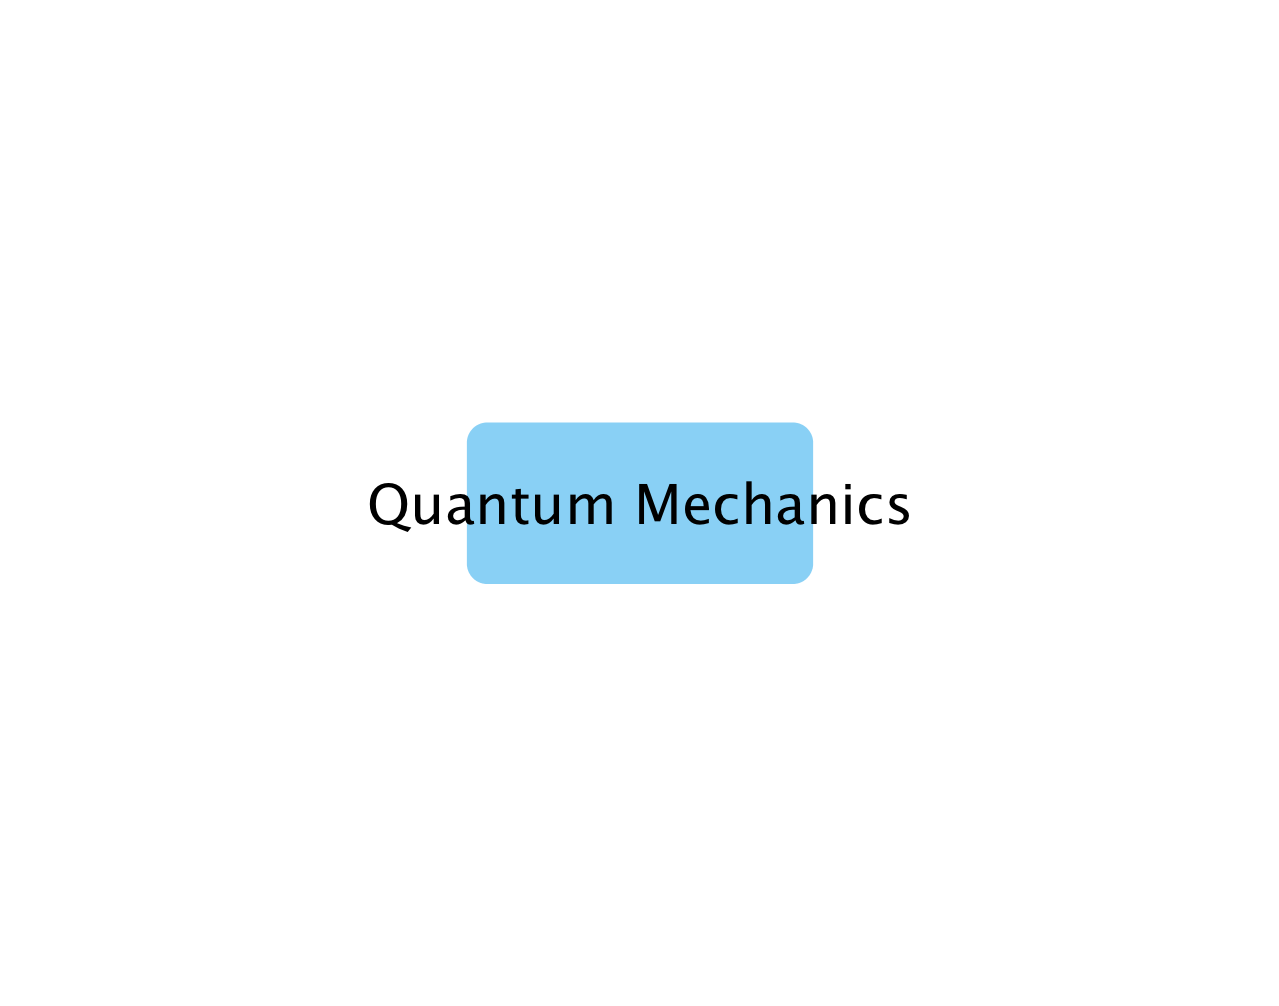
\includegraphics[width=\textwidth]{Resources/QuantumMechanics_v_1_e_0.png}
        \caption{\fontsize{10pt}{12pt}\selectfont A graph containing a single Wikipedia page (node)}
\label{fig:Node}
    \end{subfigure}
    ~ %add desired spacing between images, e. g. ~, \quad, \qquad, \hfill etc.
      %(or a blank line to force the subfigure onto a new line)
    \begin{subfigure}[b]{0.45\textwidth}
        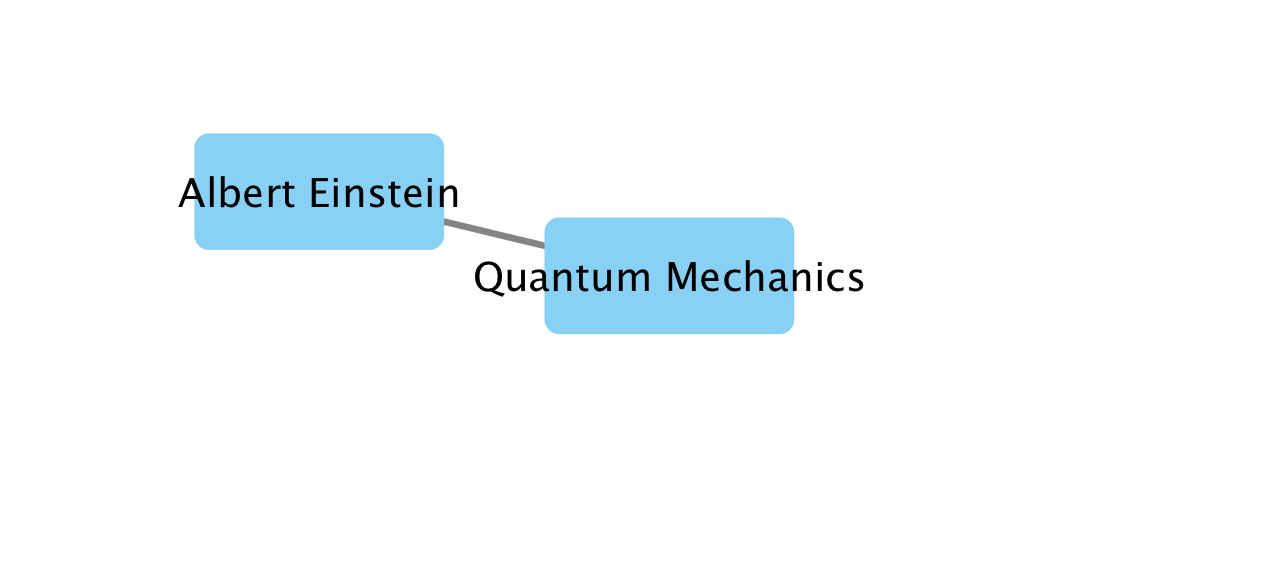
\includegraphics[width=\textwidth]{Resources/QuantumMechanics_v_2_e_1.png}
        \caption{\fontsize{10pt}{12pt}\selectfont A graph containing two Wikipedia pages (nodes), one of
        which is linked to the other (represented by the edge
        drawn between the two nodes)}
\label{fig:NodesAndLink}
    \end{subfigure}
    \caption[Basic Graph Theory Example]{\fontsize{10pt}{12pt}\selectfont Application of basic Graph Theory concepts to
    mapping the links on Wikipedia pages}\label{fig:GraphTheoryExample}
\end{figure}
\subsection{Relevant Software}
The process of mapping Wikipedia pages can be reduced to a relatively simple
algorithm, shown in Listing~\ref{lst:Psudocode}.  First, identify a
page---Quantum Mechanics, in this case---to map: \lstinline[language=Python]|page_name = "Quantum Mechanics"|. Next, retrieve all of the links on
that page: \lstinline[language=Python]|page_links = get_links_on_page(page_name)|.  Then, create a
graph that represents the relationship between the page being mapped and its
links: \lstinline[language=Python]|graph = make_graph(page_name, page_links)|.  Finally, create a
visual representation of the graph: \lstinline[language=Python]|draw(graph)|.  While it would be
possible
to implement this algorithm by hand, manually searching through Wikipedia pages
and drawing graphs of the connections between pages by hand, I chose to use several
pieces of software which simplified the algorithm's implementation.
\begin{lstlisting}[caption={Psudocode implementation of the basic mapping algorithm},label={lst:Psudocode},language=Python]
  page_name = "Quantum Mechanics"
  page_links = get_links_on_page(page_name)
  graph = make_graph(page_name, page_links)
  draw(graph)
\end{lstlisting}
The first
step of the process---identifying a page to map---does not require any
additional software to implement.  For steps 2-3---retrieving the links on the
page and making a graph of the connections---I used the Python programming
language.  To automate retrieving lists of the links on a Wikipedia page, I
used the \emph{wikipedia} package \parencite{Goldsmith2014}, while for constructing graphs of the
connections, I used the \emph{igraph} package \parencite{Csardi2006}.
Finally, for the 4th step---creating visualizations of graphs---I used the
Cytoscape program \parencite{Cytoscape}. All of the visualizations in this
paper were produced using Cytoscape.  When this algorithm is applied to the
links on an entire
Wikipedia page, the result is a graph
like that displayed in Figure \ref{fig:QuantumMechanics_v_618_e_617_b}, with
all of the nodes representing
links on the page connected to the node representing the source page (in Figure
\ref{fig:QuantumMechanics_v_618_e_617_b}, the source page is Quantum Mechanics).
\begin{figure}[!b]
  \centering
    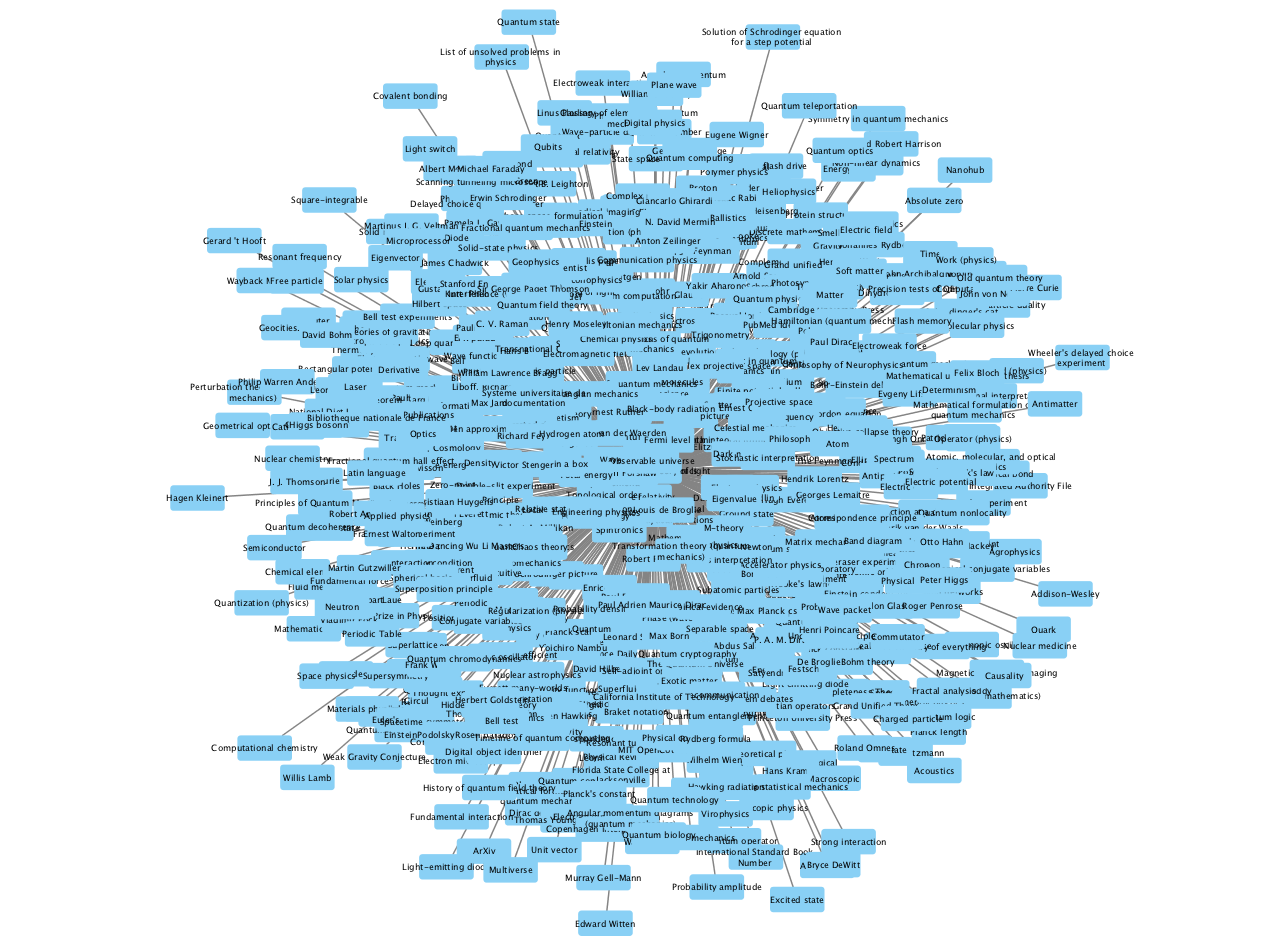
\includegraphics[width=6in, height=3.5in]{Resources/nolimit/1iteration/QuantumMechanics_v_618_e_617_b.png}
  \captionof{figure}[Quantum Mechanics Graph (1 iteration) - layout 1]{\fontsize{10pt}{12pt}\selectfont Graph of
  links on Wikipedia's Quantum Mechanics page.  Displayed with Cytoscape's
  Perfuse Force-Directed Layout (OpenCL-Accelerated)
    \label{fig:QuantumMechanics_v_618_e_617_b}}
\end{figure}

While the version of the algorithm outlined above is a good starting place, it
only allows us to see the links displayed on a single page.  One of the most promising
applications of visualizations of the connections between Wikipedia pages is that they would allow
users to trace ``paths'' through the pages, helping users understand the way
different concepts and ideas are related.  In order to do this, the algorithm
needs to be generalized to add the links found on the pages linked to by the original page and so
forth, over multiple iterations.  The process of generalizing the basic
algorithm displayed above is not easily explained in psudocode; however, the complete
Python code for the generalized algorithm is provided in Appendix B.  This
generalized version of the algorithm allows for the creation of graphs like the
one displayed in Figure \ref{fig:QuantumMechanics_v_45656_e_175822_b}, which is the result of running the algorithm
for two iterations on the Quantum Mechanics page: the graph contains all of the
links on the Quantum Mechanics page and all of the links found on the pages
linked to by the Quantum Mechanics page.  Figure \ref{fig:QuantumMechanics_v_45656_e_175822_b} contains 45,656 pages and
175,822 links between pages.
\begin{figure}[]
  \centering
    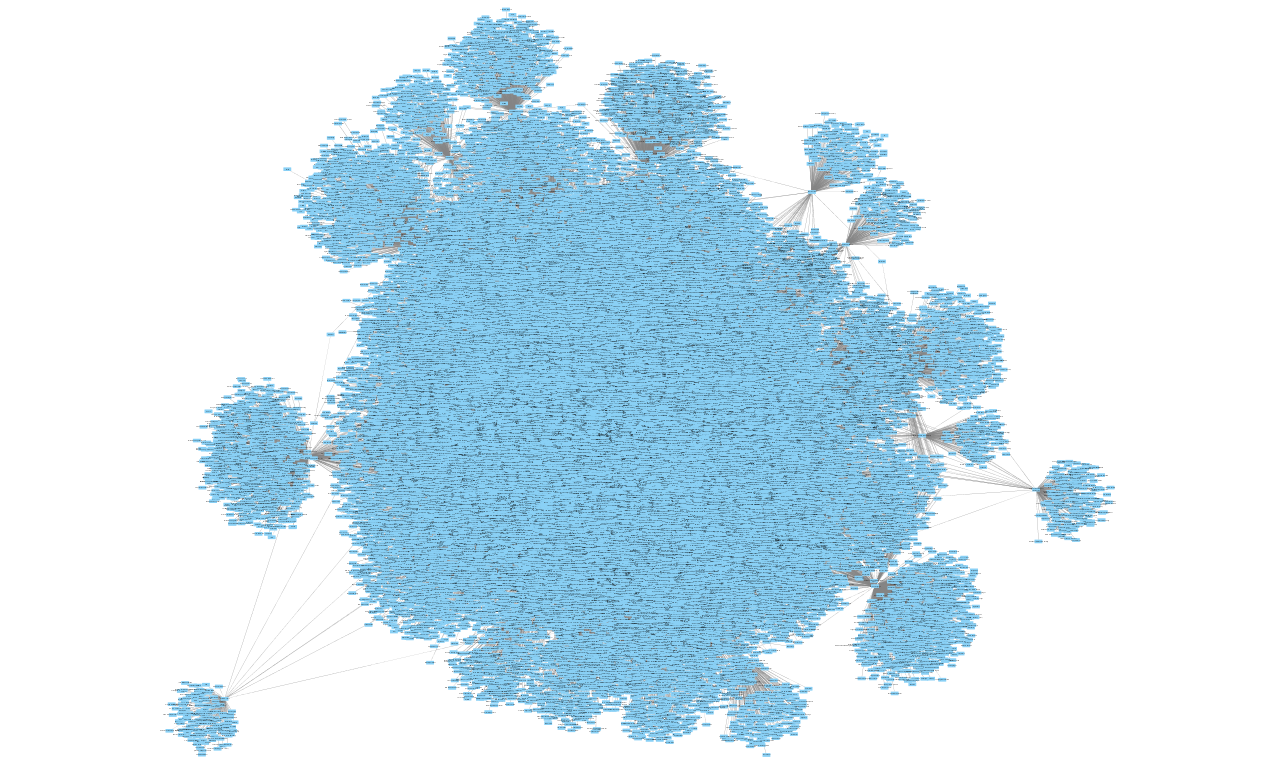
\includegraphics[width=6in, height=3.5in]{Resources/nolimit/2iterations/QuantumMechanics_v_45656_e_175822_nolimit_b.png}
  \captionof{figure}[Quantum Mechanics Graph (2 iterations) - layout 2]{Graph of links on Wikipedia's Quantum Mechanics page after 2
  iterations of the mapping algorithm.  Displayed with Cytoscape's Perfuse Force-Directed Layout (OpenCL-Accelerated)
    \label{fig:QuantumMechanics_v_45656_e_175822_b}}
\end{figure}

\section{Limitations of the First Implementation}
There are some obvious limitations to this implementation.  The graph,
even after only two iterations of the algorithm, is far too large for a user to interact
with.  Another consequence of the massive size of the graph is that it does
not display easily in web browsers, which would be the ideal medium to deploy
these visualizations. Some graph drawing algorithms also struggle with the
task of laying out large graphs; an example of what can go wrong with large
graphs and certain layout algorithms is provided in Appendix C.  Additionally,
running the algorithm for only two
iterations does not capture all of the interactions between ideas that I hope
these visualizations can display.

Looking forward to future implementations, perhaps the simplest way to improve
the utility of these visualizations is
to find a way to reduce the number of nodes in the graph.  If, instead of
displaying
600+ links per page, it were only necessary to display 10, the visualizations
would be much more manageable to interact with---both from a human perspective
and in terms of the computational overhead.
\begin{figure}
    \centering
    \begin{subfigure}[b]{0.3\textwidth}
        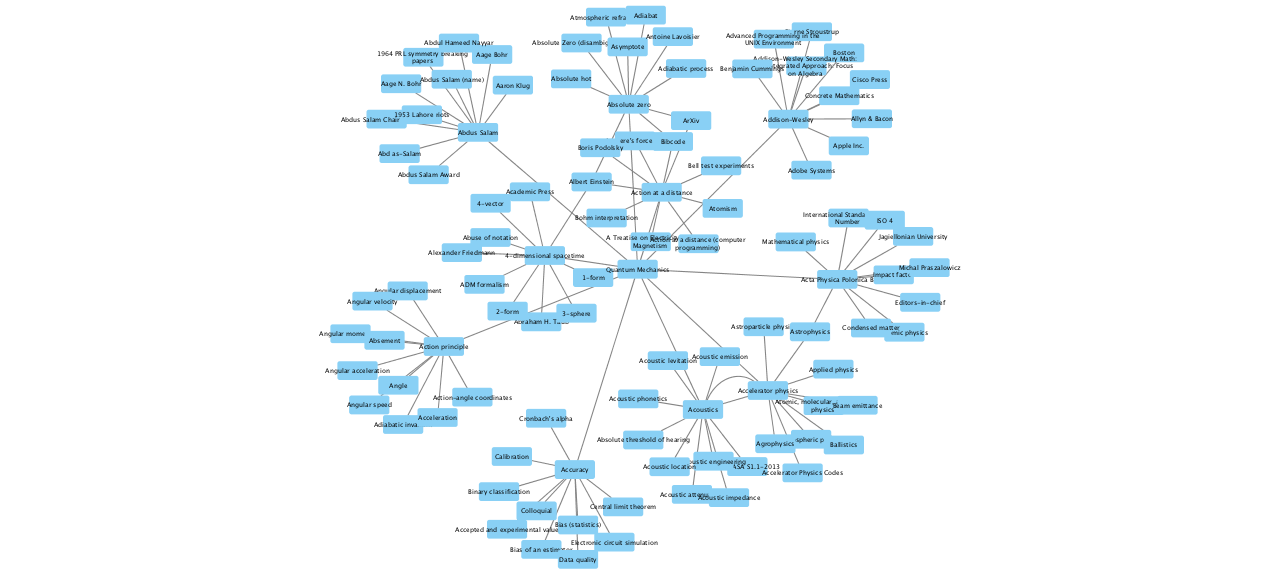
\includegraphics[width=\textwidth]{Resources/10max/2iterations/QuantumMechanics_v_104_e_110_b.png}
        \caption{\fontsize{10pt}{12pt}\selectfont Reduced graph of links on the
        Quantum Mechanics page after 2 iterations of the mapping algorithm}
        \label{fig:2iterations}
    \end{subfigure}
    \begin{subfigure}[b]{0.3\textwidth}
        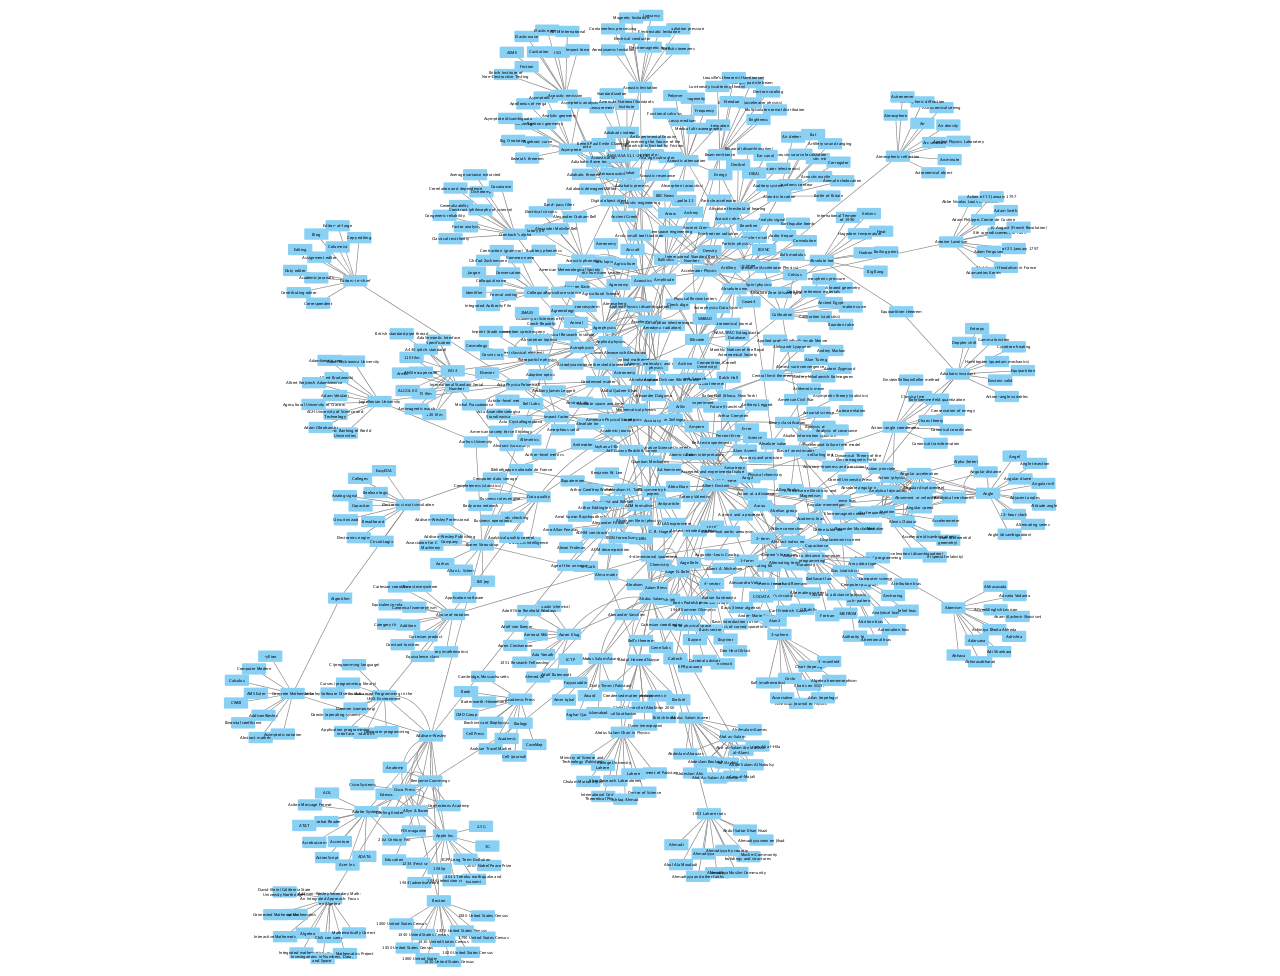
\includegraphics[width=\textwidth]{Resources/10max/3iterations/QuantumMechanics_v_717_e_1009_b.png}
        \caption{\fontsize{10pt}{12pt}\selectfont Reduced graph of links on the
        Quantum Mechanics page after 3 iterations of the mapping algorithm}
        \label{fig:3iterations}
    \end{subfigure}
    \begin{subfigure}[b]{0.3\textwidth}
        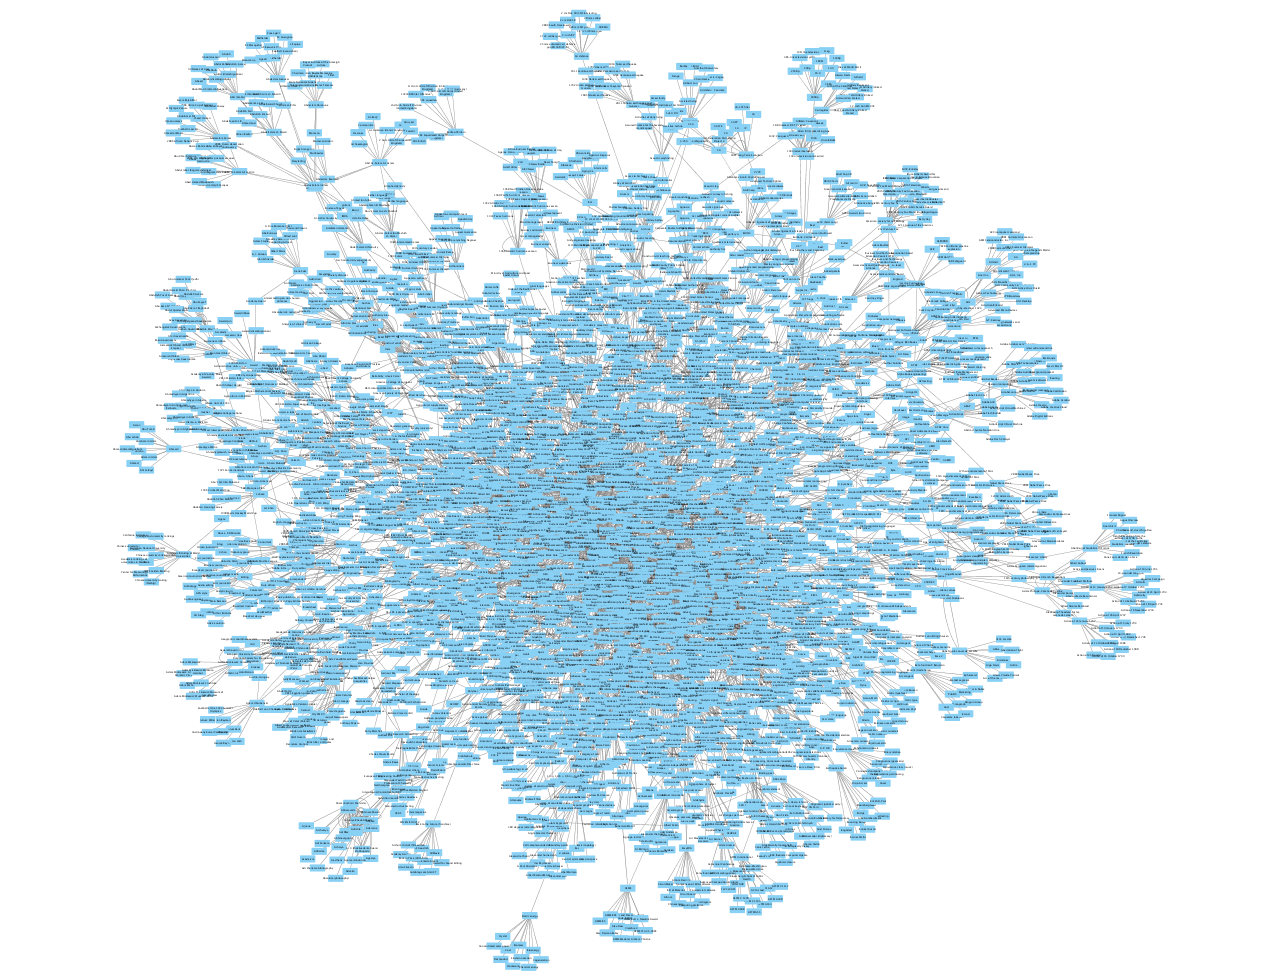
\includegraphics[width=\textwidth]{Resources/10max/4iterations/QuantumMechanics_v_3924_e_6891_b.png}
        \caption{\fontsize{10pt}{12pt}\selectfont Reduced graph of links on the
        Quantum Mechanics page after 4 iterations of the mapping algorithm}
        \label{fig:4iterations}
    \end{subfigure}
    \caption[Examples of reduced graphs]{\fontsize{10pt}{12pt}\selectfont Reduced graph of links on the
    Quantum Mechanics page after various iterations of the mapping algorithm.
    Displayed with Cytoscape's Perfuse Force-Directed Layout (OpenCL-Accelerated)}\label{fig:LimitedGraphs}
\end{figure}
This filtering could be implemented by using machine
learning algorithms such as language modeling to determine which links are the most important for understanding the
content on a page.  For the purpose of showing the utility of having fewer links per page, I have simulated this filtering by limiting the number each
page's links to 10; the graphs for 2, 3, and 4 iterations of the algorithm are
included in Figure \ref{fig:LimitedGraphs}.  Even after 4 iterations of the
algorithm, there are
only 3924 nodes and 6891 edges in the reduced graph---one and two orders of magnitude,
respectively, fewer nodes and edges than were present in the Quantum Mechanics
graph after only two iterations when no limit was placed on how many edges
each node can have.  Once the number of nodes in the graph has been reduced,
then it also becomes important to look at different ways to display the
graphs---that is, to explore the different graph layout algorithms that exist.
Appendix A includes visualizations of several different graph layout algorithms
applied to a graph of the same Wikipedia page.

Though the first implementation produces graphs which are not possible to
interact with, I think this project has a promising future.  Mitra's research
suggests there is a great latent potential for self organized learning in youth.
Future versions of maps of Wikipedia---incorporating online bodies of
Procedural and Strategic knowledge and applying machine learning algorithms
to determine which links on Wikipedia are most important to understanding
a concept---could help tap this latent potential.  Eventually, these visualizations
could help students---in both formal and informal settings---chart their own
paths through human knowledge.


% \begin{figure}[h]
%   \centering
%     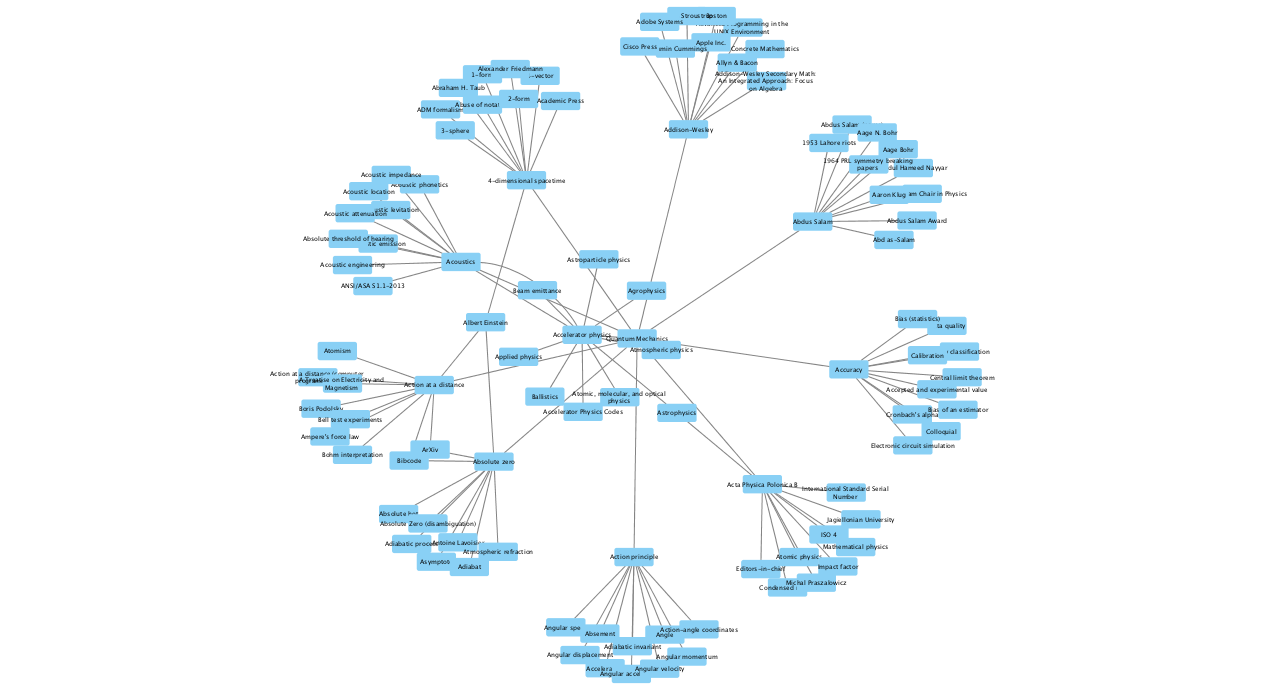
\includegraphics[width=6in, height=3.5in]{Resources/10max/2iterations/QuantumMechanics_v_104_e_110_a.png}
%   \captionof{figure}[Reduced Quantum Mechanics Graph (2 iterations) - layout 1]{Reduced (10 links per page) graph of links on Wikipedia's Quantum Mechanics page after 2
%   iterations of the mapping algorithm.  Displayed with Cytoscape's Organic Layout
%     \label{figQuantumMechanics_v_104_e_110_a}}
% \end{figure}


\appendix
\section{Comparison of Different Graph Layouts in Cytoscape}
\addcontentsline{toc}{section}{Appendix A: Comparison of Different Graph Layouts in Cytoscape}
% a: Cytoscape Organic Layout
\begin{figure}[h]
  \centering
    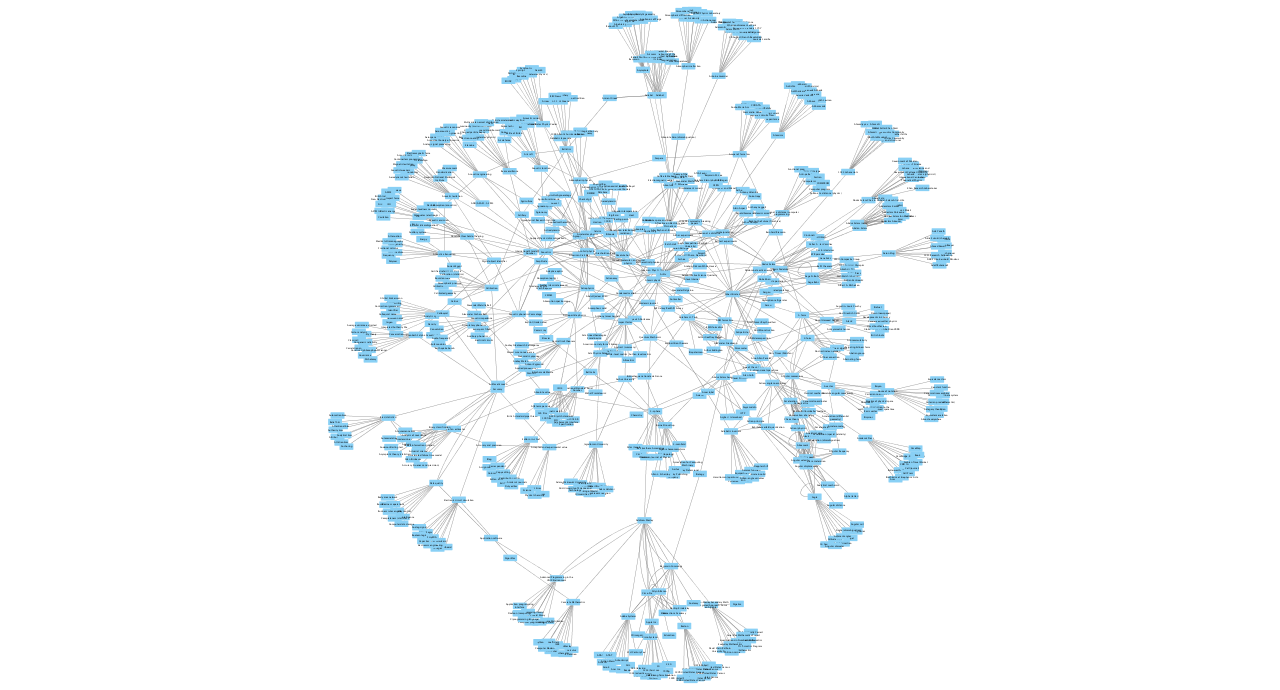
\includegraphics[width=6in, height=3in]{Resources/10max/3iterations/QuantumMechanics_v_717_e_1009_a.png}
  \captionof{figure}[Reduced Quantum Mechanics Graph (3 iterations) - layout 1]{Reduced (10 links per page) graph of links on Wikipedia's Quantum Mechanics page after 3
  iterations of the mapping algorithm.  Displayed with Cytoscape's Organic Layout
    \label{figQuantumMechanics_v_717_e_1009_a}}
\end{figure}
% b: Cytoscape Perfuse Force-Directed Layout (OpenCL-Accelerated)
\begin{figure}[h]
  \centering
    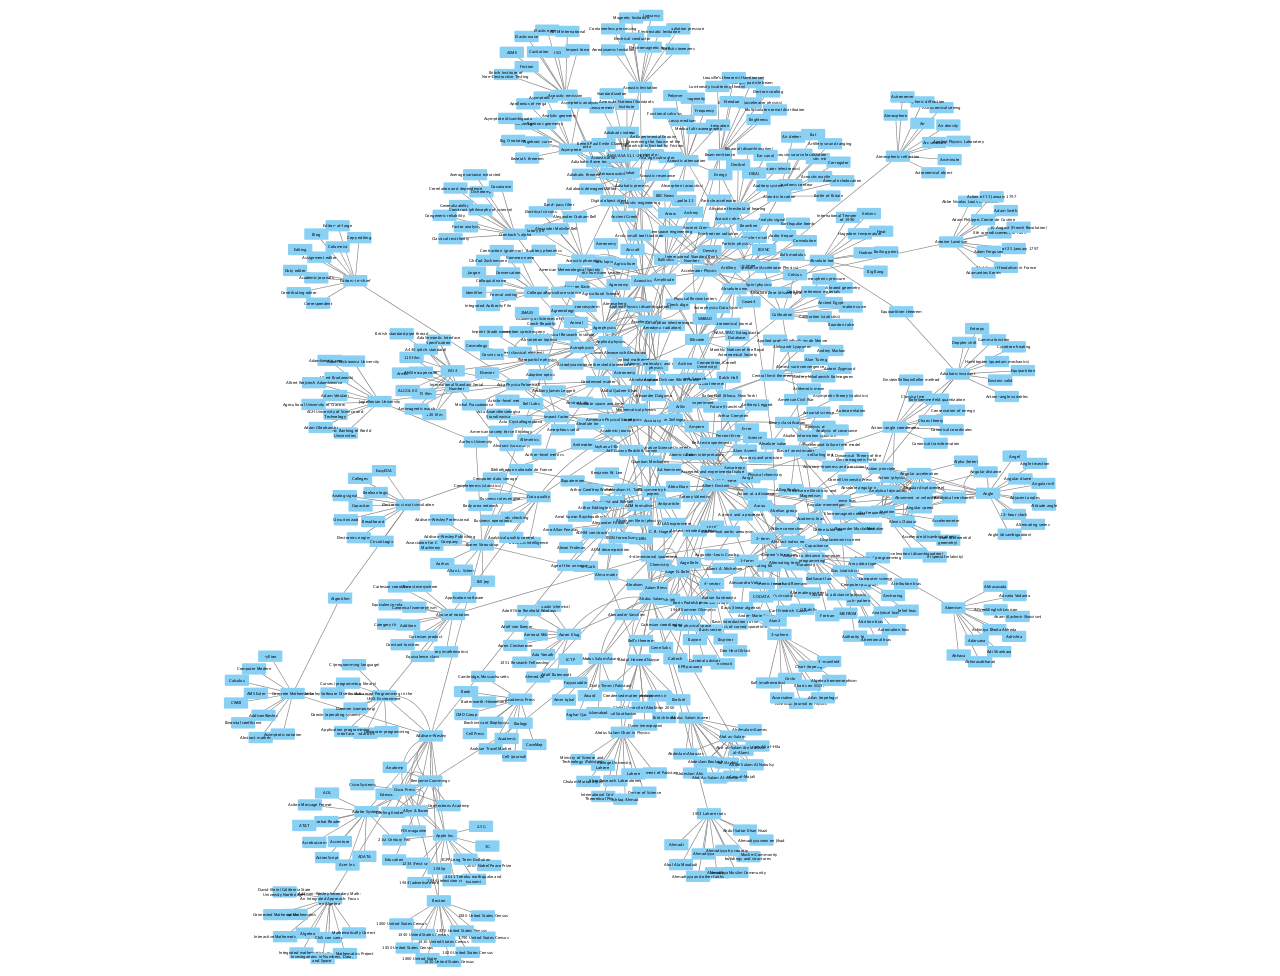
\includegraphics[width=6in, height=3in]{Resources/10max/3iterations/QuantumMechanics_v_717_e_1009_b.png}
  \captionof{figure}[Reduced Quantum Mechanics Graph (3 iterations) - layout 2]{Reduced (10 links per page) graph of links on Wikipedia's Quantum Mechanics page after 3
  iterations of the mapping algorithm.  Displayed with Cytoscape's Perfuse Force-Directed Layout (OpenCL-Accelerated)
    \label{figQuantumMechanics_v_717_e_1009_b}}
\end{figure}
% c: Cytoscape Perfuse Force-Directed Layout
\begin{figure}[h]
  \centering
    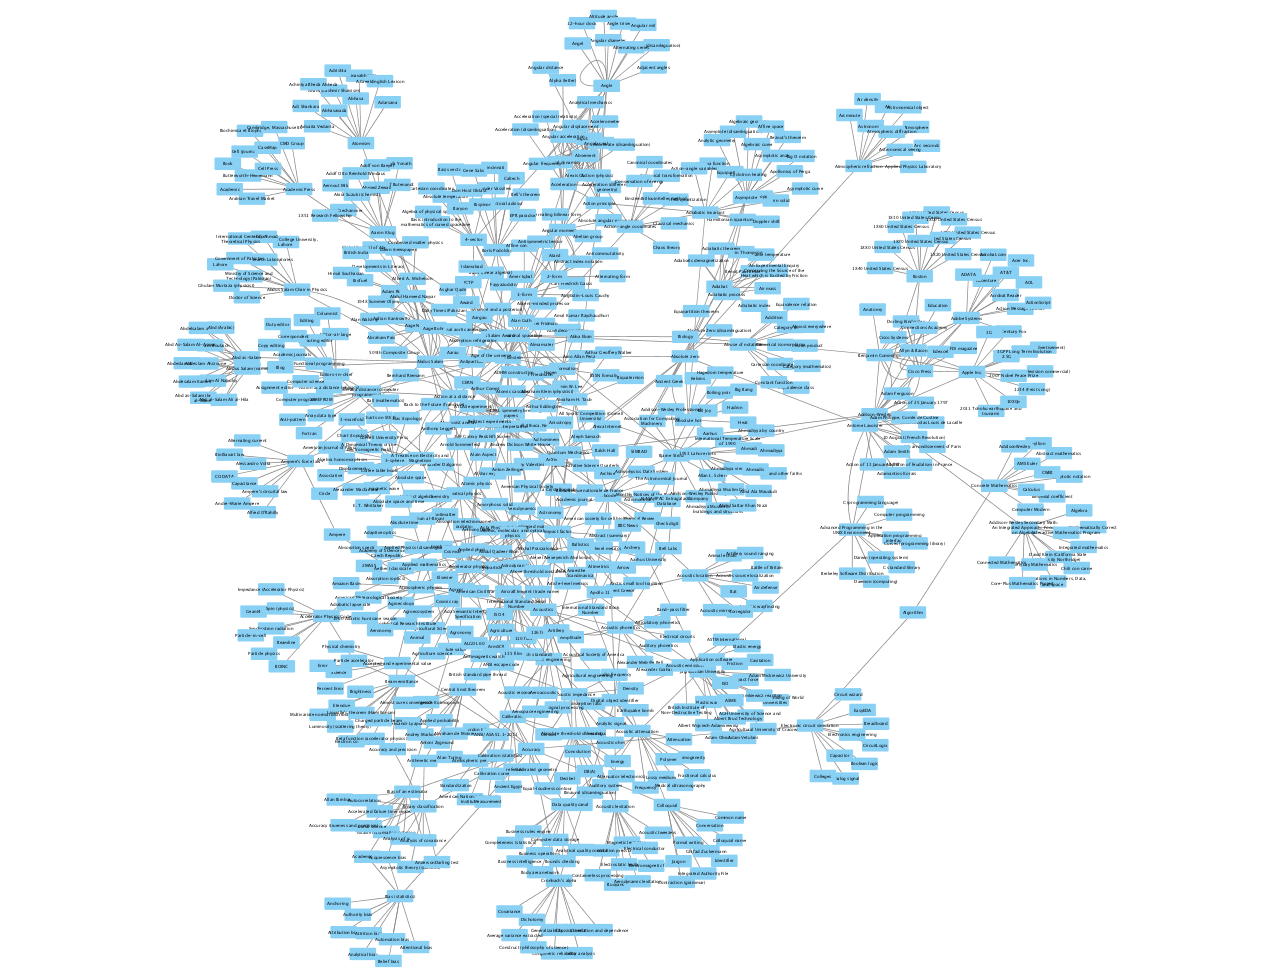
\includegraphics[width=6in, height=3in]{Resources/10max/3iterations/QuantumMechanics_v_717_e_1009_c.png}
  \captionof{figure}[Reduced Quantum Mechanics Graph (3 iterations) - layout 3]{Reduced (10 links per page) graph of links on Wikipedia's Quantum Mechanics page after 3
  iterations of the mapping algorithm.  Displayed with Cytoscape's Perfuse Force-Directed Layout
    \label{figQuantumMechanics_v_717_e_1009_c}}
\end{figure}

\section{Python Code Used to Generate GraphML Files}
\addcontentsline{toc}{section}{Appendix B: Python Code Used to Generate GraphML Files}
\begin{lstlisting}[language=Python, caption=Complete Python Implementation of
  the Mapping Algorithm]
import wikipedia
import igraph
import unicodedata

class WikipediaGraph(igraph.Graph):
    def __init__(self, start_page, num_iterations=1):
        igraph.Graph.__init__(self)
        self.start_page = start_page
        self.num_iterations = num_iterations
        self.unicode_errors = []
        self.add_page_to_graph(self.start_page)
    def is_page_in_graph(self, page_name):
        """
            Checks whether a page named "page_name" is in the graph
        """
        page_vertex = None
        try:
            page_vertex = self.vs.find(name=page_name)
            return True
        except ValueError:
            return False
    def is_page_mapped(self, page_name):
        """
            Checks whether page "page_name" has been mapped
        """
        if self.is_page_in_graph(page_name) == False:
            return False
        if self.vs.find(name=page_name)["is_mapped"] == False:
            return False
        return True
    def add_page_to_graph(self, page_name):
        max_map = 1000
        count = 1
        page = None
        try:
            page = wikipedia.page(page_name)
        except (wikipedia.DisambiguationError, wikipedia.PageError) as e:
            print page_name
            return
        print page_name
        page_links = map(lambda x: unicodedata.normalize('NFKD', x).encode('ascii','ignore'), page.links)
        # if page isn't in graph
        if self.is_page_in_graph(page_name) == False:
            self.add_vertex(name = page_name) # add the page to the graph
            self.vs.find(name = page_name)["is_mapped"] = True
            for link in page_links:
                if count > max_map:
                    break
                count += 1
                if self.is_page_in_graph(link) == False: # if the target page isn't already in the graph
                    link_vertex = self.add_vertex(name = link)
                    self.vs.find(name = link)["is_mapped"] = False
                self.add_edge(page_name, link) # connects the source and target pages
        # if page is in graph but hasn't been mapped
        if self.is_page_mapped(page_name) == False and self.is_page_in_graph(page_name) == True:
            self.vs.find(name = page_name)["is_mapped"] = True
            for link in page_links:
                if count > max_map:
                    break
                count += 1
                if self.is_page_in_graph(link) == False: # if the target page isn't already in the graph
                    link_vertex = self.add_vertex(name = link)
                    self.vs.find(name = link)["is_mapped"] = False
                self.add_edge(page_name, link) # connectes the source and target pages
        if self.is_page_mapped(page_name) == True and self.is_page_in_graph(page_name) == True:
            return
    def write(self):
        file_name = "{}_v_{}_e_{}.graphml".format(self.start_page, self.vcount(), self.ecount())
        print file_name
        return super(WikipediaGraph, self).write(file_name, format="graphml")

if __name__ == "__main__":
    num_iterations = 2
    current_iteration = 1
    g = WikipediaGraph("Quantum Mechanics")
    while current_iteration <= num_iterations:
        current_vertices = igraph.VertexSeq(g).select(is_mapped=False)[:]
        for v in current_vertices:
            g.add_page_to_graph(v["name"])
        current_iteration += 1
        g.write()
\end{lstlisting}
\section{Problems with Large Graph Layouts}
% \begin{figure}[]
%   \centering
%     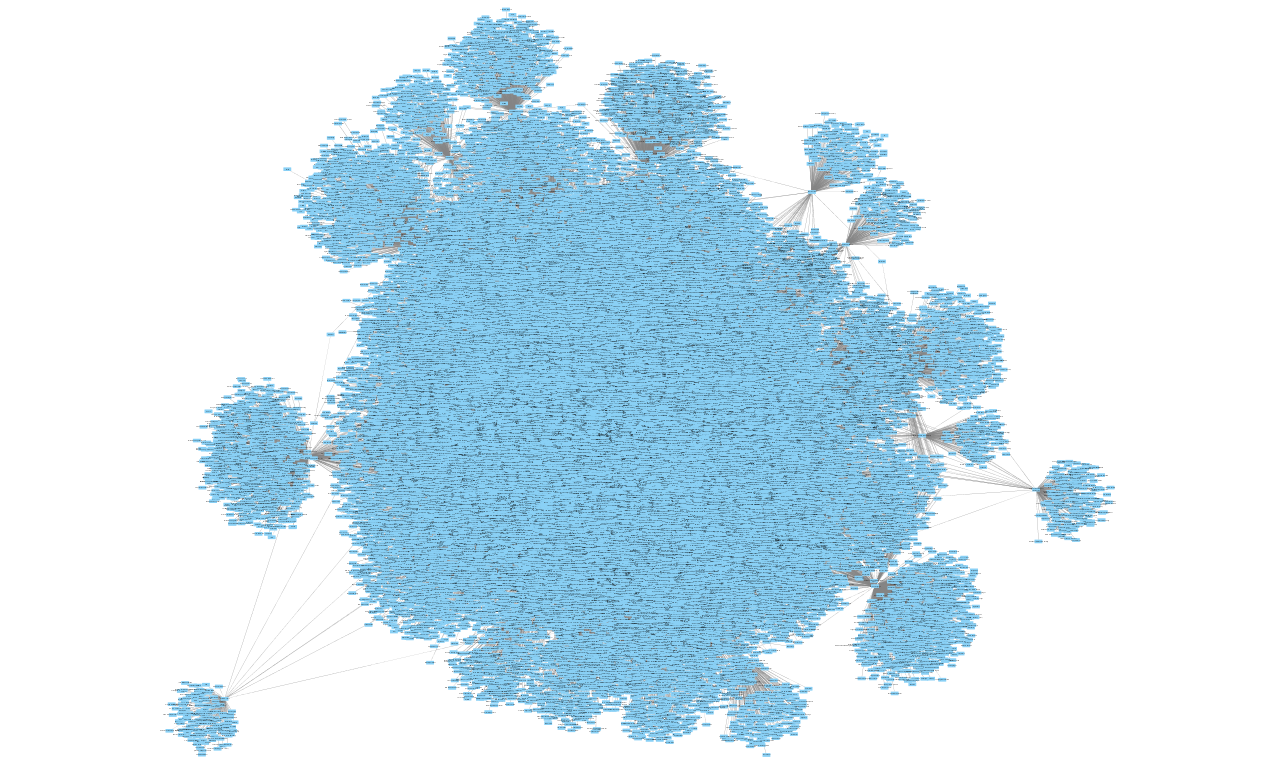
\includegraphics[width=6in, height=3.5in]{Resources/nolimit/2iterations/QuantumMechanics_v_45656_e_175822_nolimit_b.png}
%   \captionof{figure}[Successful large graph layout]{Example of a successful large graph layout.  Displayed with Cytoscape's Perfuse Force-Directed Layout (OpenCL-Accelerated)
%     \label{fig:largeSuccess}}
% \end{figure}
\begin{figure}[]
  \centering
    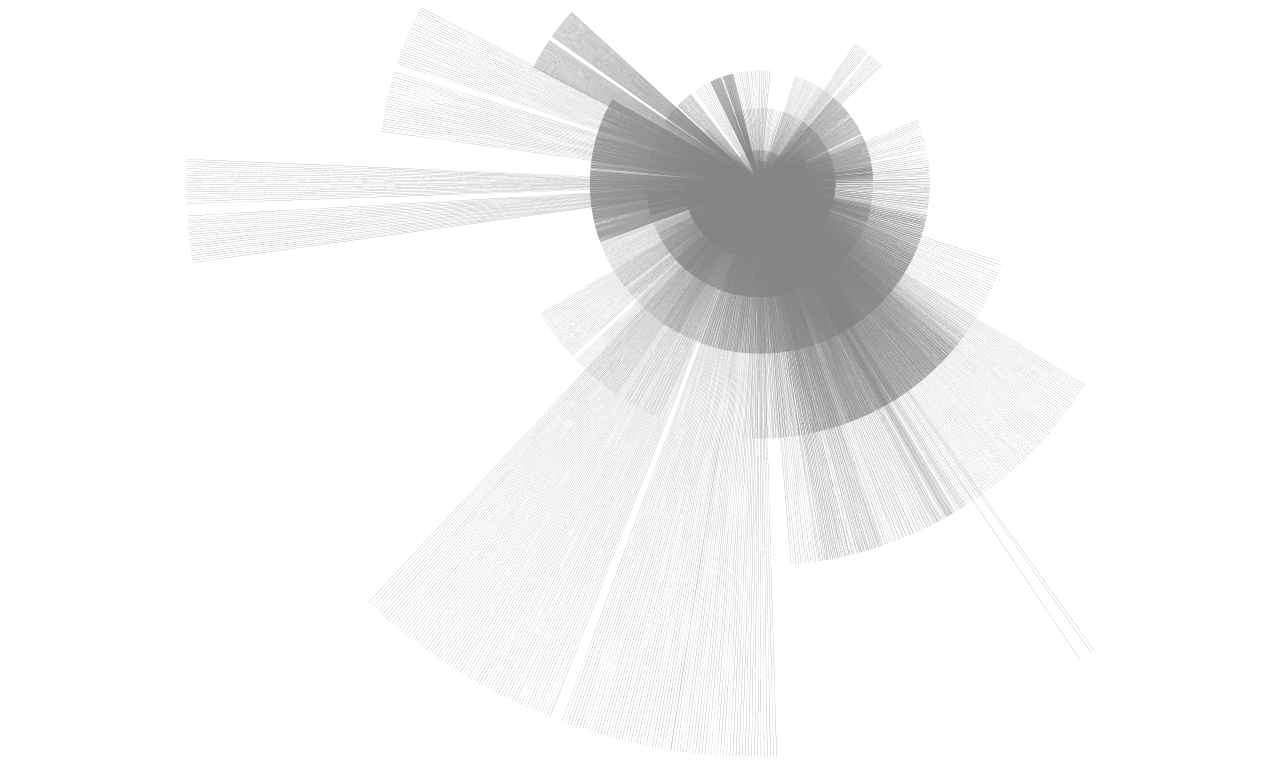
\includegraphics[width=6in, height=3.5in]{Resources/nolimit/2iterations/QuantumMechanics_v_45656_e_175822_nolimit_a.png}
  \captionof{figure}[Unsuccessful large graph layout]{Example of an unsuccessful large graph layout.  Displayed with Cytoscape's Organic Layout
    \label{fig:largeSuccess}}
\end{figure}

\nocite{*}
\printbibliography[heading=bibnumbered]
\addcontentsline{toc}{section}{References}
\end{document}

%%%%%%%%%%%%%%%%%%%%%%%%%%
%%%%%%%%%%%%%%%%%%%%%%%%%%
%% End Document Content %%
%%%%%%%%%%%%%%%%%%%%%%%%%%
%%%%%%%%%%%%%%%%%%%%%%%%%%
